

% \section{inleiding}%
% Aan de hand van de shortlist die opgemaakt is komt er voor elke geselecteerde managementplatform een proof of concept. Hierbij wordt er gekeken hoe de nodige functionaliteiten werken en toegepast kunnen worden in het systeem.
% Belangrijk om te weten is dat de proof of concept niet de volledige functionaliteit van het managementplatform zal testen. Het doel is om een goed beeld te krijgen van de mogelijkheden en hoe deze kunnen worden toegepast binnen de infrastructuur van Excentis. 
% We verdelen alle managementplatformen in hun eigen subsecties. In deze subsecties worden dan de vooropgestelde testen op uitgevoerd.
% \section{Proxmox VE}%

% Voor deze virtual managementplatform wordt er Proxmox VE 8.4 gebruikt. Dit is de laatste versie van Proxmox VE die op dit moment beschikbaar is.
\subsection{cluster opstelling in Proxmox VE}
Voor proxmox VE is er gekozen om te werken met 3 fysieke node's. Zoals beschreven op de officiële documentatiepagina van Proxmox ondersteunt het platform high availability clustering maar moeten er minimaal 3 nodes in de cluster draaien ~\autocite{proxmoxHA}.
Hierbij spreken we over minimaal 50\% van de nodes die moeten draaien om de cluster operationeel te houden. Dit is ook de reden waarom er voor 3 nodes is gekozen.
Bij 2 nodes zou er bij een node failure geen quorum zijn en zou de cluster niet meer operationeel zijn. Dit wil zeggen dat er geen 50\% meerderheid is van de cluster die online is. Enkel bij 3 nodes kan er 1 node uitvallen en alsnog meer dan 50 procent online hebben. In zo een gavel spreken we van een quorum.
In de figuur \ref{fig:cluster-proxmox} wordt de opstelling getoond. Elke node heeft zijn unieke naam in de cluster, vaak is dat de hostname zelf.
\begin{figure}[H]
  \centering
  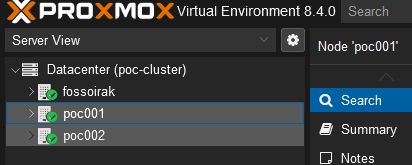
\includegraphics[width=0.85\textwidth]{../poc/cluster-info-prox.png}
  \caption{Clusteropstelling in Proxmox VE}
  \label{fig:cluster-proxmox}
\end{figure}
\subsection{Storage in Proxmox VE}
\label{sec:storage_proxmox}
Proxmox VE ondersteunt verschillende soorten storage. In de proof of concept is er gekozen om te werken met een CEPH storage als distributed storage. Dit is een open-source software-defined storage oplossing die kan worden gebruikt in combinatie met Proxmox VE.
Om deze te configureren moeten er minimaal 3 schijven/partities zijn. Voor deze POC is er besloten om op elke fysieke node een fysieke schijf toe te kennen aan de CEPH storage. Dit zijn 3 willekeurige harde schijven.
Via de GUI kan vanaf elke node worden doorgeklikt naar Ceph. Daar moet worden aangeduid welke schijf gebruikt zal worden voor de Ceph-storage. Dit kan ook via de command line.
Nadat de schijven op elke node zijn toegevoegd, kan via het OSD-menu in de Proxmox-GUI een overzicht worden bekeken, zoals te zien is in figuur \ref{fig:osd-ceph-proxmox}.
\begin{figure}[H]
  \centering
  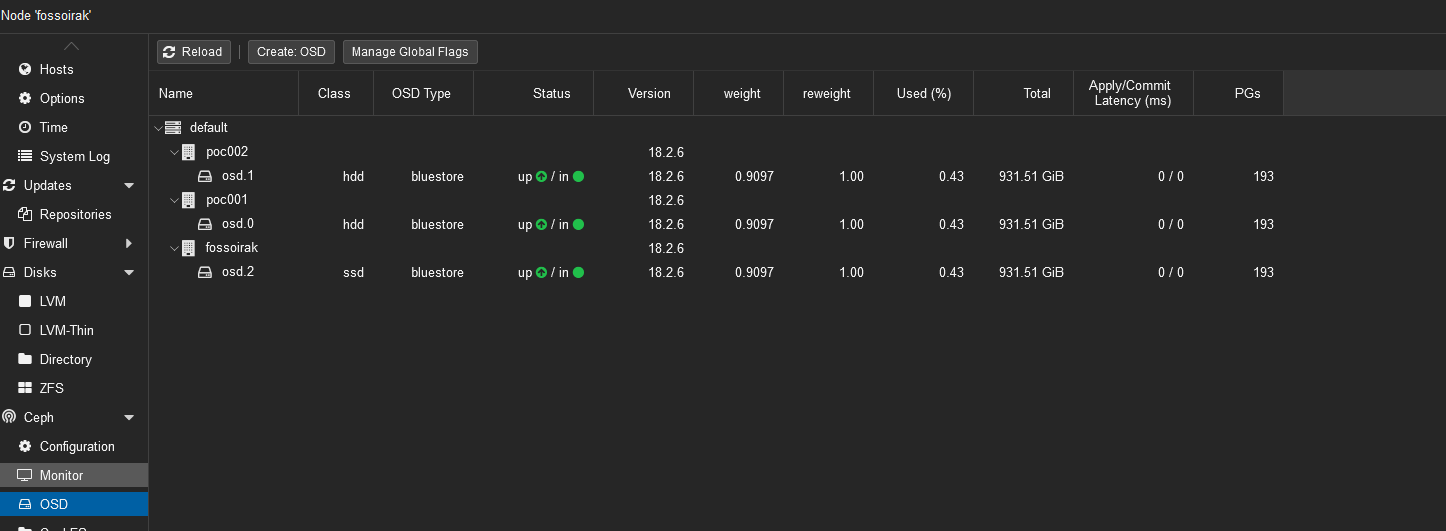
\includegraphics[width=1.2\textwidth]{../poc/ceph-osd-prox.png}
  \caption{CEPH schijven opstelling in Proxmox VE}
  \label{fig:osd-ceph-proxmox}
\end{figure}

Nu kan er een pool aangemaakt worden voor de CEPH storage. Hierin wordt het belangrijste deel van de CEPH configuratie gedaan.
Je geeft aan hoeveel schijven er in de pool moeten zitten. Minimaal is dit hier 3 aangezien we weer met het HA systeem zitten. Om de HA regels te volgen is het ook essentieel dat er op elke fysieke node een schijf zit voor de pool.
Bij het gebruik van Ceph in Proxmox VE moet het systeem weten hoeveel schijven minimaal beschikbaar moeten zijn om de opslagpool operationeel te houden. Voor deze POC wordt dit ingesteld op 2. Dit is ook de reden waarom er met 3 fysieke nodes is gewerkt. Bij een node failure kan de pool nog steeds gebruikt worden.
De Crush rule in de configuratie is ook belangrijk. Dit is de manier waarop de data verdeeld wordt over de verschillende schijven. Hierin kan ook worden aangegeven dat er een replica van de data op een andere node moet worden gemaakt. Bij een node failure kan de data nog steeds worden benaderd via de andere nodes.
De firguur \ref{fig:ceph-pool-prox} toont de huidige configuratie van de pool in Proxmox VE.
\begin{figure}[H]
  \centering
  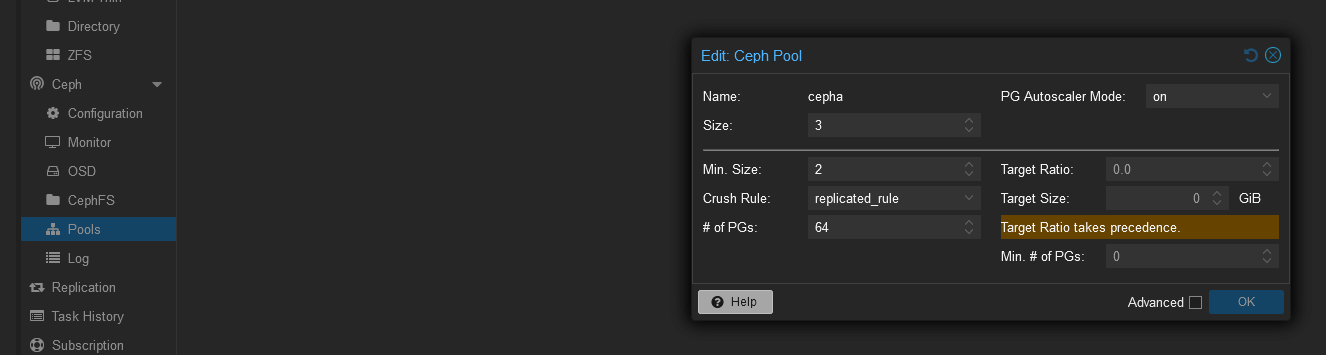
\includegraphics[width=1.1\textwidth]{../poc/ceph-pool-prox.png}
  \caption{Pool opstelling van CEPH in Proxmox VE}
  \label{fig:ceph-pool-prox}
\end{figure}

Eenmaal aangemaakt kan er een virtuele machine worden aangemakt. Deze virtuele zal Ubuntu 22.04 worden gebruikt als operating system.
De meeste instellingen kunnen helemaal naar keuze worden ingesteld en is voor de rest buiten de scope van deze bachelorproef. De meest relevante instellingen zijn die rond de storage.
Tijdens het configureren van de virtuele machine kan de gewenste schijf worden geselecteerd. Hierbij kan ook de eerder aangemaakte pool worden gekozen.
Merk verder op dat er al een optie is voor SAN iSCSI met TrueNAS~\autocite{truenas} . Deze optie mag tijdelijk genegeerd worden.
Als alles correct is verlopen, kan op alle drie de nodes naar keuze een virtuele machine worden aangemaakt, waarbij overal dezelfde optie beschikbaar is om Ceph als schijfopslag te gebruiken.
Figuur \ref{fig:vm-storage-proxmox} toont de configuratie van de virtuele machine in Proxmox VE.
\begin{figure}[H]
  \centering
  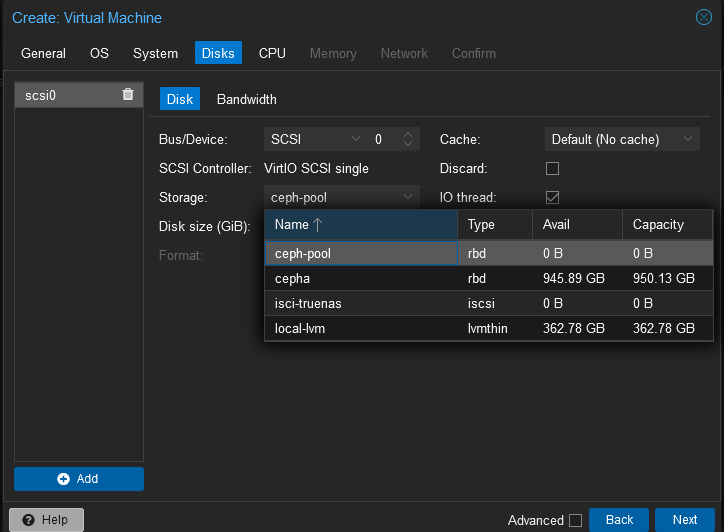
\includegraphics[width=0.85\textwidth]{../poc/vm-storage-prox.png}
  \caption{VM configuratie met correcte disk in Proxmox VE}
  \label{fig:vm-storage-proxmox}
\end{figure}

De virtuele machine is nu aangemaakt op de node fossoirak.
Ter controle kan er in de GUI onder Datacenter bij de optie CEPH gekeken worden of alle schijven en nodes die de CEPH pool draaien healthy zijn. Zie figur \ref{fig:ceph-healthy-prox}.
Als er geen rode kruisjes staan bij de schijven en nodes is alles perfect geconfigureerd.
\begin{figure}[H]
  \centering
  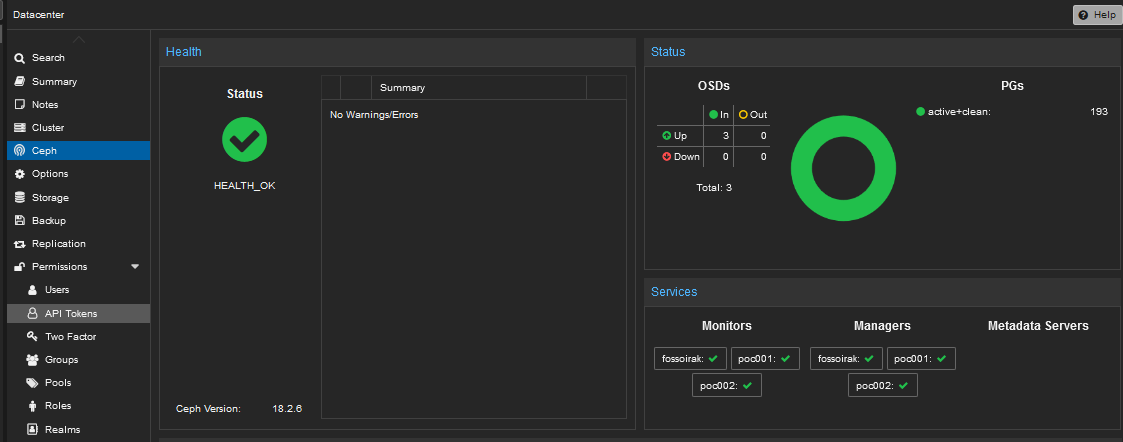
\includegraphics[width=1.1\textwidth]{../poc/ceph-healthy-prox.png}
  \caption{de gezondheid van CEPH  in Proxmox VE}
  \label{fig:ceph-healthy-prox}
\end{figure}

Hierna kan er een HA test uitgevoerd worden. Dit wordt later besproken.
Tijdens het werken met Proxmox VE valt er op dat Proxmox VE automatisch een direct attach storage mount aanmaakt voor te gebruiken. Deze wordt gekoppeld als een directory met als naam local.
Dit toont aan dat Proxmox VE standaard een integratie biedt met DAS. In deze situatie draait het direct op de schijf waar de Proxmox VE zelf op draait zoals te zien is in de figuur \ref{fig:das-prox}.
\begin{figure}[H]
  \centering
  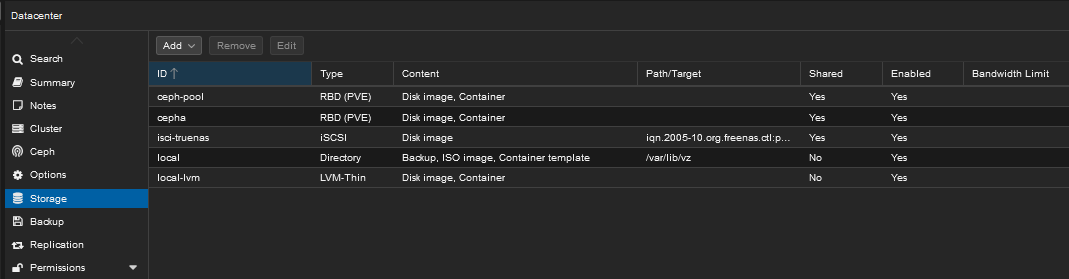
\includegraphics[width=1.2\textwidth]{../poc/das-proxmox.png}
  \caption{direct attach storage in Proxmox VE}
  \label{fig:das-prox}
\end{figure}


Nu we weten dat CEPH goed werkt moet er gekeken worden naar de SAN configuratie met ISCSI.
Er is een bestaande TrueNAS ~\autocite{truenas} server die al draait in de omgeving. Hierop draait een block storage waar iSCI is geconfigureerd.
Onder de tab storage bij Datacenter kan er zeer eenvoudig een iSCSI target worden aangemaakt bij Add, zie figuur \ref{fig:iscsi-SAN}.
Via de opties in het menu moet er een correct ID als naam worden gegeven en via portal het correct IP adres van de TrueNAS service.
Omdat er gewerkt wordt met een SAN principe staat het default bij de optie node in de configuratie op all nodes. Dit is ook de bedoeling aangezien we met een HA cluster werken.
De configuratie van iSCI op TrueNAS is buiten de scope van deze bachelorproef.
\begin{figure}[H]
  \centering
  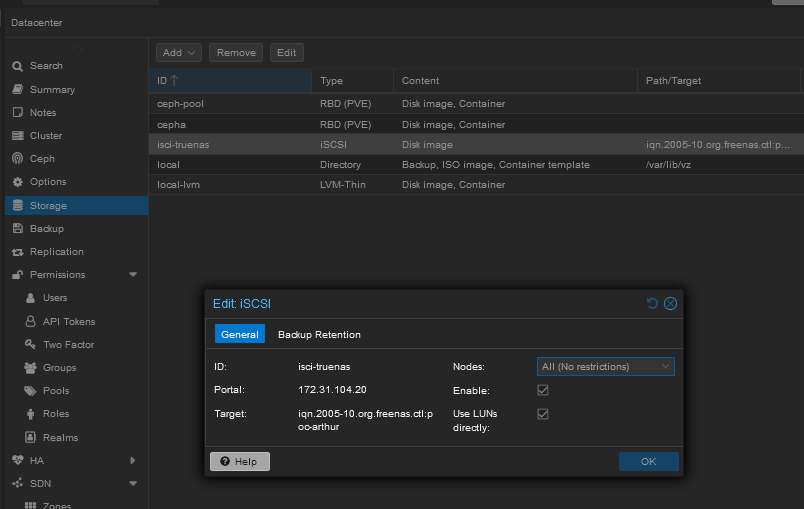
\includegraphics[width=1.1\textwidth]{../poc/iscsi-prox.png}
  \caption{storage area network met ISCI in Proxmox VE}
  \label{fig:iscsi-SAN}
\end{figure}
Nu zal er een extra  optie bijgekomen zijn in de GUI onder de tab storage bij datacenter, zie fiuur~\ref{fig:vm-lijst}  Hier in het voorbeeld wordt het al naam iSCI-TrueNAS gegeven.
Nu maken we een 2de virtuele machine aan met dezelfde configuratie als de eerste virtuele machine maar met een andere disk. Er wordt nu gekozen voor de isci-truenas disk.
\begin{figure}[H]
  \centering
  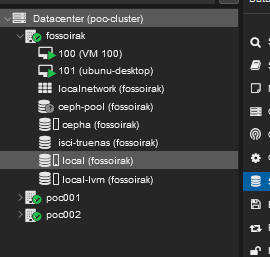
\includegraphics[width=0.85\textwidth]{../poc/vm-lijst-prox.png}
  \caption{Lijst van de 2 virtuele machines in Proxmox VE}
  \label{fig:vm-lijst}
\end{figure}
Aangezien een SAN princiepe via een vebrinding werkt op het netwerk is de storage de zwakste schakel in een high availability cluster. Deze verbinding kan verbroken worden door netwerk problemen. Hierna kan er data corruptie onstaan in het slechtste geval.

\subsection{High Availability in Proxmox VE}
\label{sec:ha-proxmox}
Eenmaal de storage in orde is voor de virtuele machines kan er een HA configuratie worden aangemaakt. 
Onder datacenter HA kan een groep worden aangemaakt. Hierin worden alle drie de fysieke nodes opgenomen die deel uitmaken van de cluster. Vervolgens wordt aan de groep een logische naam toegekend, in dit geval ha-pool zoals in figuur \ref{fig:ha-group}.
\begin{figure}[H]
  \centering
  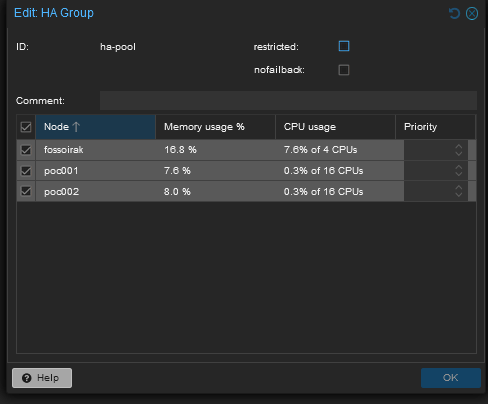
\includegraphics[width=0.85\textwidth]{../poc/ha-group.png}
  \caption{high Availability group in Proxmox VE}
  \label{fig:ha-group}
\end{figure}
Nu voegen we de 2 virtuele machines toe aan de HA groep. Dit wordt gedaan via de HA section in datancer.
Bij Max Restart en Max Relocate wordt ingesteld hoe vaak een virtuele machine opnieuw mag worden opgestart of verplaatst naar een andere node. In dit geval moet dit groter zijn dan 0 zoals bij firguur \ref{fig:ha-vm}.
\begin{figure}[H]
  \centering
  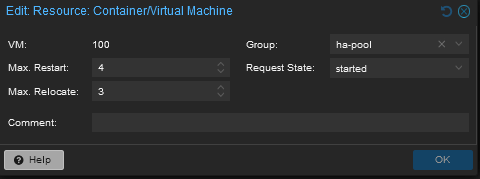
\includegraphics[width=0.85\textwidth]{../poc/vm-ha.png}
  \caption{High Availability vm toevoegen in Proxmox VE}
  \label{fig:ha-vm}
\end{figure}
% Ik heb dit verplaatst naar poc




\begin{figure}[H]
  \centering
  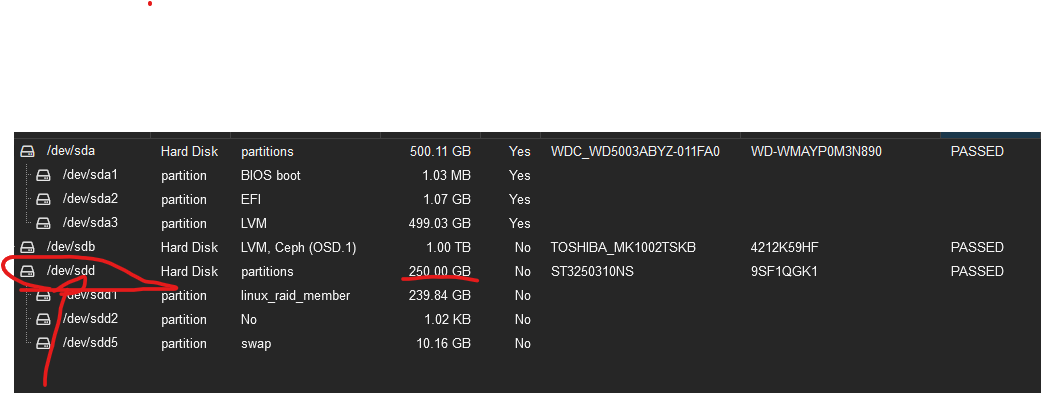
\includegraphics[width=1.2\textwidth]{../poc/hot-disktwee-prox.png}
  \caption{hot disk swap in Proxmox VE}
  \label{fig:hotdiskvervangen-swap}
\end{figure}

We zien bij figuur` \ref{fig:hotdiskvervangen-swap} dit duidelijk een andere disk is met nu een grote van 250 GB. Hiervoor was dat 500 GB.